% Options for packages loaded elsewhere
\PassOptionsToPackage{unicode}{hyperref}
\PassOptionsToPackage{hyphens}{url}
%
\documentclass[
  9pt,
  ignorenonframetext,
]{beamer}
\usepackage{pgfpages}
\setbeamertemplate{caption}[numbered]
\setbeamertemplate{caption label separator}{: }
\setbeamercolor{caption name}{fg=normal text.fg}
\beamertemplatenavigationsymbolsempty
% Prevent slide breaks in the middle of a paragraph
\widowpenalties 1 10000
\raggedbottom
\setbeamertemplate{part page}{
  \centering
  \begin{beamercolorbox}[sep=16pt,center]{part title}
    \usebeamerfont{part title}\insertpart\par
  \end{beamercolorbox}
}
\setbeamertemplate{section page}{
  \centering
  \begin{beamercolorbox}[sep=12pt,center]{part title}
    \usebeamerfont{section title}\insertsection\par
  \end{beamercolorbox}
}
\setbeamertemplate{subsection page}{
  \centering
  \begin{beamercolorbox}[sep=8pt,center]{part title}
    \usebeamerfont{subsection title}\insertsubsection\par
  \end{beamercolorbox}
}
\AtBeginPart{
  \frame{\partpage}
}
\AtBeginSection{
  \ifbibliography
  \else
    \frame{\sectionpage}
  \fi
}
\AtBeginSubsection{
  \frame{\subsectionpage}
}
\usepackage{lmodern}
\usepackage{amsmath}
\usepackage{ifxetex,ifluatex}
\ifnum 0\ifxetex 1\fi\ifluatex 1\fi=0 % if pdftex
  \usepackage[T1]{fontenc}
  \usepackage[utf8]{inputenc}
  \usepackage{textcomp} % provide euro and other symbols
  \usepackage{amssymb}
\else % if luatex or xetex
  \usepackage{unicode-math}
  \defaultfontfeatures{Scale=MatchLowercase}
  \defaultfontfeatures[\rmfamily]{Ligatures=TeX,Scale=1}
\fi
\usetheme[]{Goettingen}
\usecolortheme{rose}
% Use upquote if available, for straight quotes in verbatim environments
\IfFileExists{upquote.sty}{\usepackage{upquote}}{}
\IfFileExists{microtype.sty}{% use microtype if available
  \usepackage[]{microtype}
  \UseMicrotypeSet[protrusion]{basicmath} % disable protrusion for tt fonts
}{}
\makeatletter
\@ifundefined{KOMAClassName}{% if non-KOMA class
  \IfFileExists{parskip.sty}{%
    \usepackage{parskip}
  }{% else
    \setlength{\parindent}{0pt}
    \setlength{\parskip}{6pt plus 2pt minus 1pt}}
}{% if KOMA class
  \KOMAoptions{parskip=half}}
\makeatother
\usepackage{xcolor}
\IfFileExists{xurl.sty}{\usepackage{xurl}}{} % add URL line breaks if available
\IfFileExists{bookmark.sty}{\usepackage{bookmark}}{\usepackage{hyperref}}
\hypersetup{
  pdftitle={BIOS6643 Longitudinal},
  pdfauthor={EJC},
  hidelinks,
  pdfcreator={LaTeX via pandoc}}
\urlstyle{same} % disable monospaced font for URLs
\newif\ifbibliography
\setlength{\emergencystretch}{3em} % prevent overfull lines
\providecommand{\tightlist}{%
  \setlength{\itemsep}{0pt}\setlength{\parskip}{0pt}}
\setcounter{secnumdepth}{-\maxdimen} % remove section numbering
\AtBeginSubsection{}
\AtBeginSection{}
\ifluatex
  \usepackage{selnolig}  % disable illegal ligatures
\fi

\title{BIOS6643 Longitudinal}
\subtitle{L6 DF and DDF}
\author{EJC}
\date{}
\institute{Department of Biostatistics \& Informatics}

\begin{document}
\frame{\titlepage}

\begin{frame}[allowframebreaks]
  \tableofcontents[hideallsubsections]
\end{frame}
\hypertarget{degrees-of-freedom}{%
\section{Degrees of freedom}\label{degrees-of-freedom}}

\begin{frame}{Topics}
\protect\hypertarget{topics}{}
\begin{itemize}
\tightlist
\item
  Estimating (D)DF for inference in linear mixed models.
\end{itemize}
\end{frame}

\begin{frame}{Estimating (D)DF for inference involving \(\pmb \beta\)}
\protect\hypertarget{estimating-ddf-for-inference-involving-pmb-beta}{}
\textbf{See the course notes for more detail.}
\end{frame}

\hypertarget{background}{%
\section{Background}\label{background}}

\begin{frame}{Background}
\protect\hypertarget{background-1}{}
\begin{itemize}
\item
  Inference for fixed effects in a GLM involves creation of an ANOVA
  table that breaks down total sums of squares into sources, and then
  uses this information along with DF to construct \(t\) or \(F\)-tests
  of interest.
\item
  The GLM can be extended to longitudinal data by making adjustments to
  the ANOVA table and tests, i.e., repeated measures ANOVA. A
  multivariate GLM can also be employed, along with MANOVA, to analyze
  longitudinal data with a more flexible covariance structure.
\item
  Inference for fixed effects in the LMM generally does not involve an
  ANOVA-type approach that breaks variation down into sources (although
  in special cases, the approaches are equivalent, discussed more
  shortly). Rather, test statistics are built that are functions of
  model parameters that are typically estimated using ML or REML.
\item
  Distributions of these test statistics have approximate \(t\) or
  \(F\)-distributions (under the null hypothesis), with accuracy that
  can be calibrated by selection of the denominator degrees of freedom
  (DDF). {[}For \(t\)-tests, the quantity is just DF, for \(F\)-tests,
  it is DDF; but we just use DDF for simplicity.{]}
\end{itemize}
\end{frame}

\begin{frame}{}
\protect\hypertarget{section}{}
\begin{itemize}
\item
  For simpler data and models, DDF selection is clear and distributions
  `exact.' (E.g., RM ANOVA and the LMM with a random intercept for
  subjects.)
\item
  For more complex data and models (the usual case), the DDF need to be
  estimated to allow for accurate inference, including the calculation
  of \(p\)-values and confidence intervals. There is no clear cut or
  agreed upon method to estimate the DDF, although many of the proposed
  methods often yield similar results.
\item
  The reason why \(t\) and \(F\)-distributions are used (rather than
  standard normal and \(\chi^2\)- distributions) in inference for LMMs
  is due to the use of unknown covariance parameters in the test
  statistics.
\item
  This is a generalization of inference for a mean based on a random
  sample, using a \(t\)-test.
\item
  Along the same lines, inference for \(\pmb \beta\) in the LMM should
  take into account the fact that covariance parameters in the developed
  test statistics are estimated rather than known values. Again, this is
  a straightforward process for balanced data and simpler models, but
  not so clear beyond that. There have been several methods proposed to
  estimate DDF for test statistics in the LMM.
\end{itemize}
\end{frame}

\hypertarget{ddfm}{%
\section{DDFM}\label{ddfm}}

\begin{frame}{Small-sample vs.~asymptotic approaches}
\protect\hypertarget{small-sample-vs.-asymptotic-approaches}{}
When covariance parameters are known, inference for \(\pmb \beta\) in
the LMM can utilize standard normal and \(\chi^2\)- distributions. Even
when these parameters are unknown, inference based on standard normal
and \(\chi^2\)- distributions are fairly accurate for large sample sizes
(see Fitzmaurice et al.~(2011)). Although there is no one single widely
accepted DDF method (DDFM), they generally produce similar results and
are all likely to be much more accurate than the asymptotic approach.

\begin{block}{A description of DDFM approaches}
\protect\hypertarget{a-description-of-ddfm-approaches}{}
In SAS, there are five denominator degrees of freedom methods (DDFM)
that can be specified in the MODEL statement for PROC MIXED, which are
Containment, Between-within, Residual, Satterthwaite, and Kenward-Roger.
In R, recent packages and functions allow for application of some of
these methods. Below is a list and some detail for 6 common DDF methods;
for more detail, see SAS Help Documentation. Some examples follow the
list of definitions.
\end{block}
\end{frame}

\begin{frame}{Containment}
\protect\hypertarget{containment}{}
\begin{itemize}
\item
  Keyword CONTAIN.
\item
  The default method in SAS when there is a RANDOM statement in PROC
  MIXED (regardless of whether there is a REPEATED statement).
\item
  Not used in common R packages and functions.
\item
  If a predictor is named somewhere in the RANDOM statement, DDF is set
  to \(rank[\pmb X \pmb Z]\) associated with this named predictor.
  Otherwise, DDF is set to \(n–rank[\pmb X \pmb Z]\).
\end{itemize}
\end{frame}

\begin{frame}{Between-within}
\protect\hypertarget{between-within}{}
\begin{itemize}
\item
  Takes the residual DF and separates it into `between-subject' and
  `within-subject' components.
\item
  The default method in SAS when there is a REPEATED statement but no
  RANDOM statement. Keyword: BETWITHIN.
\item
  Not used in common R packages and functions.
\end{itemize}
\end{frame}

\begin{frame}{Residual}
\protect\hypertarget{residual}{}
\begin{itemize}
\item
  This is comparable to using the DF for the MSE in standard GLM, but is
  usually not recommended since it tends to overestimate the optimal DF.
  Keyword: RES.
\item
  DDF= \(n–rank[\pmb X]\).
\end{itemize}
\end{frame}

\begin{frame}{Satterthwaite}
\protect\hypertarget{satterthwaite}{}
\begin{itemize}
\item
  Performs a general Satterthwaite approximation to the DDF.
\item
  More conservative than Containment and Between-Within methods,
  although for many data sets it will be the same or similar. Keyword:
  SATTERTH or SAT.
\item
  Method available in R (e.g., \textbf{emmeans()} function).
\end{itemize}
\end{frame}

\begin{frame}{Kenward-Roger}
\protect\hypertarget{kenward-roger}{}
\begin{itemize}
\item
  Also an `approximate' method. It is an adjustment to the Satterthwaite
  approach that does even more to account for uncertainty in unknown
  covariance parameters; offers a correction to DF as well as the
  standard error in test statistics.
\item
  From data I have analyzed, DDF appears to be the same as for
  Satterthwaite, but adjusts the SE, as mentioned above.
\item
  SAS suggests this method when there is a REPEATED statement with
  TYPE=UN, but no RANDOM statement). Keyword: KENWARDROGER or KR.
\item
  Method available in R (e.g., \textbf{emmeans()} function).
\end{itemize}
\end{frame}

\begin{frame}{Asymptotic}
\protect\hypertarget{asymptotic}{}
\begin{itemize}
\item
  Uses `Infinite' DDF, i.e., uses the standard normal in place of the
  \(t\)-distribution and the \(\chi^2\)- distribution in place of the
  \(F\)-distribution.
\item
  Correct approach if the covariance parameters are known.
\item
  Not recommended if you have software that allows for inference based
  on \(t\) and \(F\)-distribution methodology, although for larger
  sample sizes there will not be big differences.
\end{itemize}
\end{frame}

\begin{frame}{DDF in SAS}
\protect\hypertarget{ddf-in-sas}{}
\begin{itemize}
\item
  You can select your own denominator degrees of freedom using DDF= in
  SAS. Thus, if you feel you have a method that gives you an even better
  approximation to the null distribution through specification of the
  denominator DF, you can specify it.
\item
  See Verbeke and Molenberghs, \emph{Linear Mixed Models in Practice,
  Springer, 1997}, Appendix A, and the SAS Help Documentation for more
  detail.
\end{itemize}
\end{frame}

\begin{frame}{Summary}
\protect\hypertarget{summary}{}
\begin{enumerate}
\item
  Residual and Asymptotic approaches are usually not recommend since
  they will likely yield \(p\)-values too small and CI's too narrow
  (i.e., approaches are too liberal).
\item
  Containment and Between-Within methods are SAS defaults.
\item
  R has the approximate approaches (Satterthwaite and Kenward-Roger) but
  often sets Asymptotic as the default.
\item
  From my experience, The Containment, Between-Within, Satterthwaite and
  Kenward-Roger are often similar in most cases, if not the same, with
  Satterthwaite and KR slightly more conservative.
\item
  But there are a few caveats to this, which are mentioned with the
  examples below. Generally, any of these four methods should be
  reasonable, and multiple approaches could be taken to verify that end
  results do not differ much between the approaches.
\end{enumerate}
\end{frame}

\hypertarget{examples}{%
\section{Examples}\label{examples}}

\begin{frame}[fragile]{Fitness data}
\protect\hypertarget{fitness-data}{}
\begin{itemize}
\item
  10 \(Subjects\) (identified using the ID variable) were randomized to
  one of two fitness \(Groups\) (5 per \(Group\)), observed over 5
  \(Times\) and evaluated for fitness levels.
\item
  Data were modeled using \(Group\), \(Time\) and \(Group \times Time\),
  using \(Group\) and \(Time\) as class variables. Thus, the degrees of
  freedom are 1 for \(Intercept\), 1 for \(Group\), 4 for \(Time\), and
  4 for \(Group \times Time\).
\item
  Recall that with RM ANOVA (refer to section here), there are 32 DDF
  for \(Time\) and \(Group \times Time\), and 8 DDF for \(Group\).
\item
  The denominator MS for \(Time\) and \(Group \times Time\) is the MSE,
  while it is \(MS_{Subject(Group)}\) for \(Group\).
\item
  For the model that uses a random intercept for \(Subject\), there are
  10 columns in the complete-data\(\pmb Z\) matrix, but 2 of these
  columns are redundant in the \([\pmb{X Z}]\) (8 d.f. related to
  \(Group\) within \(\pmb Z\)), so \(rank[\pmb {XZ}]=18\), and
  \(n–rank[\pmb {XZ}]=32\). If the random statement is written as

\begin{verbatim}
RANDOM intercept / subject=ID;
\end{verbatim}
\end{itemize}
\end{frame}

\begin{frame}[fragile]{}
\protect\hypertarget{section-1}{}
There is no predictor in the statement. Thus, \(Group\), \(Time\) and
\(Group \times Time\) \(F\)-tests will all use 32 DDF for the
Containment method (the default).

\begin{itemize}
\item
  Now if we use the following statement instead:

\begin{verbatim}
  RANDOM intercept / subject=ID(group);
\end{verbatim}
\end{itemize}

The \(Group\) variable will be recognized when using the Containment
method, which has 8 d.f. (see above). Thus, the DDF for \(Group\) will
be 8 and 32 for the others. This is one of the important caveats alluded
to previously. Since the other methods (BW, Satterthwaite and KR) all
have 8 d.f. for \(Group\) (as would the RM ANOVA) without using
ID(\(Group\)), it seems important to use ID(\(Group\)) as the
\(Subject\) if the default Containment is used.

\begin{itemize}
\tightlist
\item
  One difference between methods is that inference for
  \(Group \times Time\) combinations (e.g., Leas\(t\)-squares means
  estimates) is that the Satterthwaite and KR approaches have 11 DF for
  \(Group \times Time\) estimates (via `Least squares means' analysis)
  compared with Containment and BW approaches (32 DF). The table below
  shows composite results, including incomplete data, to show impact of
  missing data on results.
\end{itemize}
\end{frame}

\begin{frame}{}
\protect\hypertarget{section-2}{}
\begin{block}{Table 1: Estimated (D)DF for Fitness data, model with
random intercept for \(Subjects\), \(Time\) as class; unrestricted data
is balanced.}
\protect\hypertarget{table-1-estimated-ddf-for-fitness-data-model-with-random-intercept-for-subjects-time-as-class-unrestricted-data-is-balanced.}{}
\begin{center}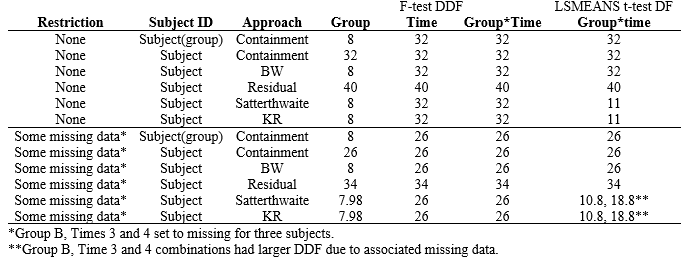
\includegraphics[width=1\linewidth]{figs_L6/t1} \end{center}
\end{block}
\end{frame}

\begin{frame}{Beta Carotene data}
\protect\hypertarget{beta-carotene-data}{}
\begin{itemize}
\item
  Each \(Subject\) is given one of four vitamin supplements and beta
  plasma levels are observed over 5 \(Times\), for 23 \(Subjects\).
  There are 6 \(Subjects\) in each \(Group\) except one that has 5.
  There are \(23 \times 5=115\) total observations. Although data are
  not balanced, they are complete, and results are similar to the
  Fitness data (see table).
\item
  For the basic GLM that does not account for repeated measures, there
  are 20 model DF (1 for \(Intercept\), 3 for \(Group\), 4 for \(Time\),
  12 for \(Group \times Time\); both \(Group\) and \(Time\) are modeled
  as class variables here). Thus, there are 95 residual DF.
\end{itemize}
\end{frame}

\begin{frame}{}
\protect\hypertarget{section-3}{}
Table 2 shows DDF values for different methods. The results show that if
you are going to use the Containment method, you should use
\(Subject(Group)\) as the `subject' in the RANDOM statement in order to
get the proper 19 DF. Recall that if the effect of interest is not in
the RANDOM statement, the DF for the Containment approach defaults to
\(n–rank[\pmb {XZ}]\). This is fine for \(Time\) and
\(Group \times Time\), but \(Group\) should have 19 DF. If a random
slope for \(Time\) is included for \(Subjects\), the Containment method
becomes similar to Satterthwaite and KR, while BW is more liberal for
\(Time\) and \(Group \times Time\). For \(t\)-tests, the DF is the same
as for \(F\)-tests for all methods except for Satterthwaite and KR when
the model has random terms for intercept and time.

\begin{block}{Table 2: Esitmated (D)DF for Beta Carotene data (complete
data, unbalanced between groups). For LSMEANS, not all combinations were
examined.}
\protect\hypertarget{table-2-esitmated-ddf-for-beta-carotene-data-complete-data-unbalanced-between-groups.-for-lsmeans-not-all-combinations-were-examined.}{}
\begin{center}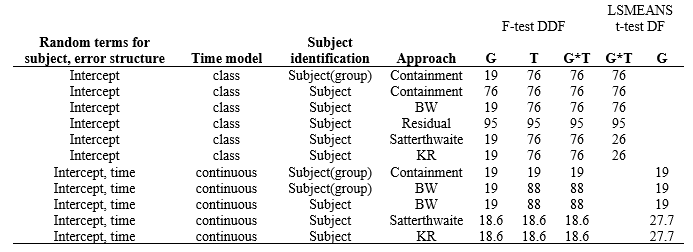
\includegraphics[width=0.8\linewidth]{figs_L6/t2} \end{center}
\end{block}
\end{frame}

\begin{frame}{}
\protect\hypertarget{section-4}{}
Table 3 illustrates differences in quantities used for \(F\)-tests. Note
that in all cases, the Numerator DF for \(Group\), \(Time\), and
\(Group \times Time\) are 3, 4, and 12. The standard GLM is clearly not
the correct approach, but used to show what happens when the
longitudinal data are not taken into account and it is assumed that
responses all came from separate \(Subjects\).

For all reasonable approaches (all but the Standard GLM), results are
pretty similar, except for the \(Group \times Time\) \(p\)-value using
the Satterthwaite method when both a random intercept and AR(1)
structure for the error covariance structure are in the model, in which
case a lower DDF elevates the \(p\)-value above 0.05. Even though the
Residual method is generally not recommended, it does not yield results
too different from others, even though the total sample size is just
over 100.

\begin{block}{Table 3: Esitmated DDF for Beta Carotene, \(F\) and
\(p\)-values for different models and DDFM approaches Group Time
\(Group \times Time\)}
\protect\hypertarget{table-3-esitmated-ddf-for-beta-carotene-f-and-p-values-for-different-models-and-ddfm-approaches-group-time-group-times-time}{}
\begin{center}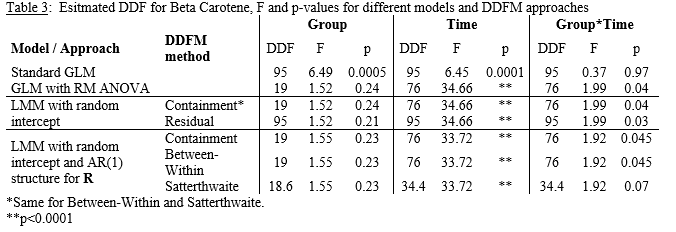
\includegraphics[width=0.8\linewidth]{figs_L6/t3} \end{center}
\end{block}
\end{frame}

\end{document}
